%Notes by Harsh Mistry 
%CS 349
%Based on Template From  https://www.cs.cmu.edu/~ggordon/10725-F12/template.tex

\documentclass[twoside]{article}
\setlength{\oddsidemargin}{0.25 in}
\setlength{\evensidemargin}{-0.25 in}
\setlength{\topmargin}{-0.6 in}
\setlength{\textwidth}{6.5 in}
\setlength{\textheight}{8.5 in}
\setlength{\headsep}{0.75 in}
\setlength{\parindent}{0 in}
\setlength{\parskip}{0.1 in}
\usepackage{amsmath,amsfonts,graphicx}
\newcounter{lecnum}
\renewcommand{\thepage}{\thelecnum-\arabic{page}}
\renewcommand{\thesection}{\thelecnum.\arabic{section}}
\renewcommand{\theequation}{\thelecnum.\arabic{equation}}
\renewcommand{\thefigure}{\thelecnum.\arabic{figure}}
\renewcommand{\thetable}{\thelecnum.\arabic{table}}
\newcommand{\lecture}[4]{
   \pagestyle{myheadings}
   \thispagestyle{plain}
   \newpage
   \setcounter{lecnum}{#1}
   \setcounter{page}{1}
   
   
%Info Box 
   \begin{center}
   \framebox{
      \vbox{\vspace{2mm}
    \hbox to 6.28in { {\bf CS 349 - User Interfaces
	\hfill Winter 2018} }
       \vspace{4mm}
       \hbox to 6.28in { {\Large \hfill Lecture #1: #2  \hfill} }
       \vspace{2mm}
       \hbox to 6.28in { {\it Lecturer: #3 \hfill Notes By: #4} }
      \vspace{2mm}}
   }
   \end{center}
   
   \markboth{Lecture #1: #2}{Lecture #1: #2}



 
}

\renewcommand{\cite}[1]{[#1]}
\def\beginrefs{\begin{list}%
        {[\arabic{equation}]}{\usecounter{equation}
         \setlength{\leftmargin}{2.0truecm}\setlength{\labelsep}{0.4truecm}%
         \setlength{\labelwidth}{1.6truecm}}}
\def\endrefs{\end{list}}
\def\bibentry#1{\item[\hbox{[#1]}]}

\newcommand{\fig}[3]{
			\vspace{#2}
			\begin{center}
			Figure \thelecnum.#1:~#3
			\end{center}
	}
	
\graphicspath{ {images/} }

\newtheorem{theorem}{Theorem}[lecnum]
\newtheorem{lemma}[theorem]{Lemma}
\newtheorem{ex}[theorem]{Example}
\newtheorem{proposition}[theorem]{Proposition}
\newtheorem{claim}[theorem]{Claim}
\newtheorem{corollary}[theorem]{Corollary}
\newtheorem{definition}[theorem]{Definition}
\newenvironment{proof}{{\bf Proof:}}{\hfill\rule{2mm}{2mm}}
\newcommand\E{\mathbb{E}}


%Start of Document 
\begin{document}

\lecture{6}{January 15, 2018}{Keiko Katsuragawa}{Harsh Mistry}

\section{Java Basics}

\subsection{Background}
\begin{itemize}
\item Designed by James Gosling
\item Released by Sun in 1995
\item Made open source in 2007
\item Acquired by Oracle in 2010
\item Portable through virtualization  
\item Class-based, object-oriented design
\end{itemize}


\subsection{Java Portability through Virtualization}
\begin{center}
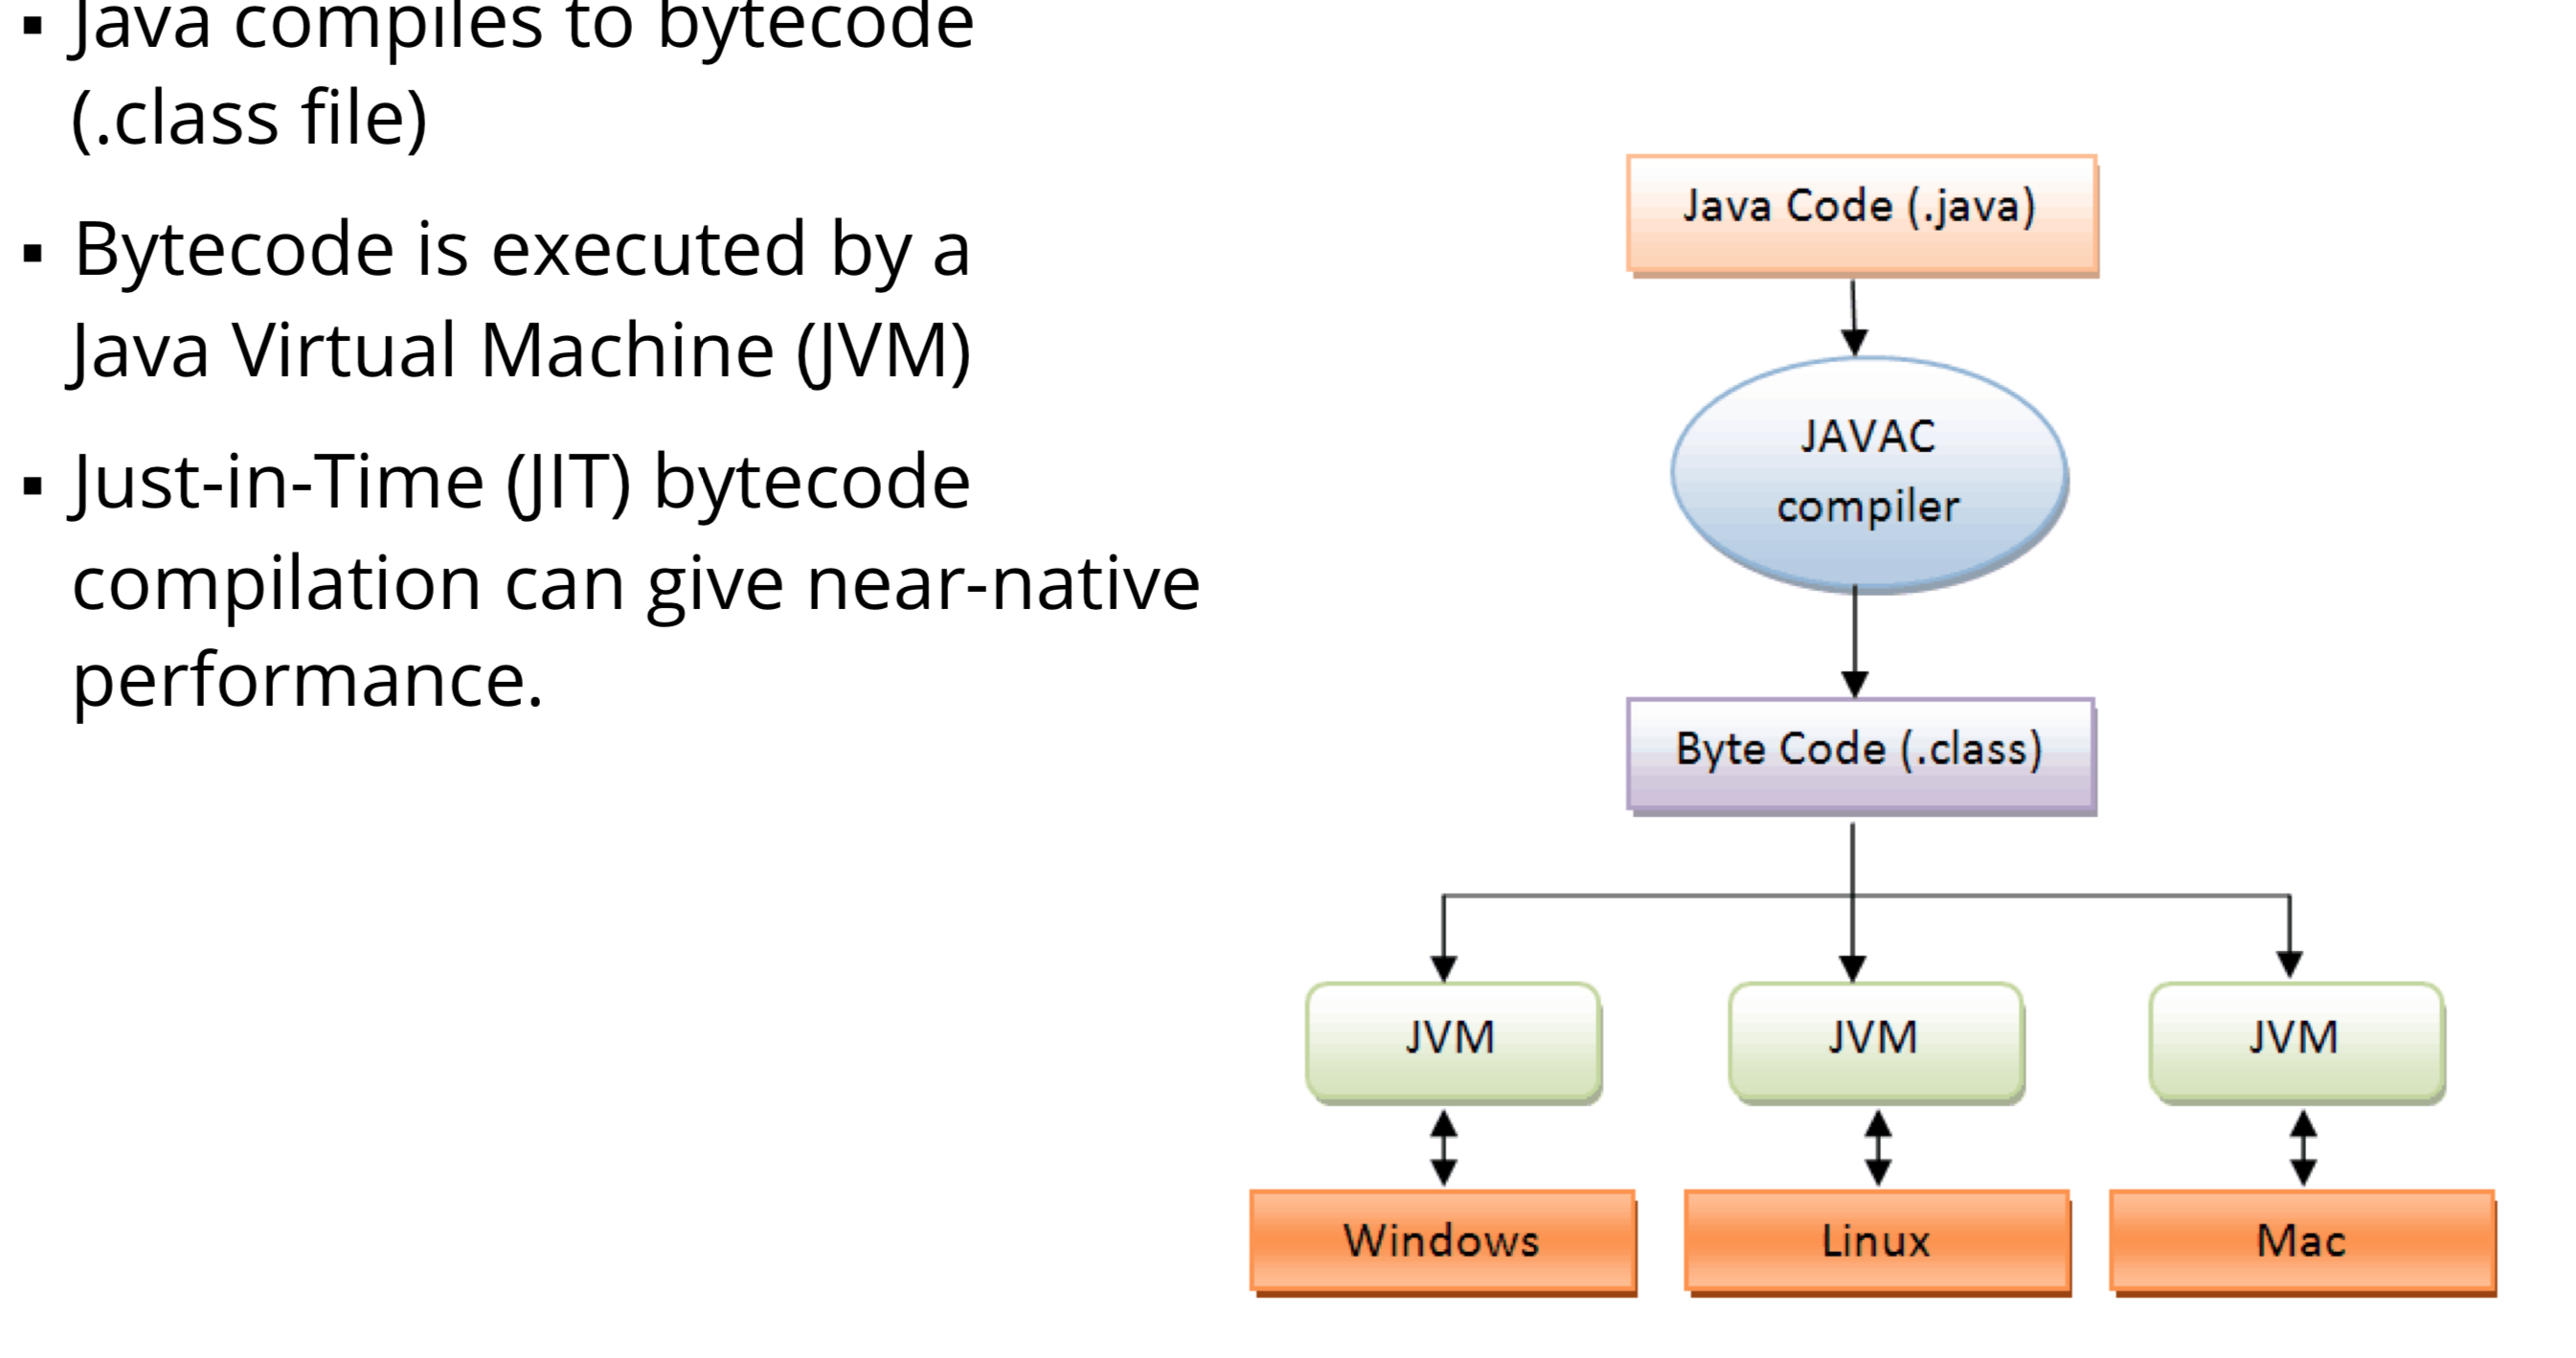
\includegraphics[scale=0.2]{10}\\
Taken from Lecture Notes
\end{center}


\subsection{Java Class Library}
\begin{itemize}
\item Classes are grouped into "packages"
\item \verb|package| keyword to assign source to a package
\item Typically, a package is a subdirectory
\item \verb|import| keyword to include a class from a different package
\end{itemize}

\subsection{Common Classes/Packages}
\begin{center}
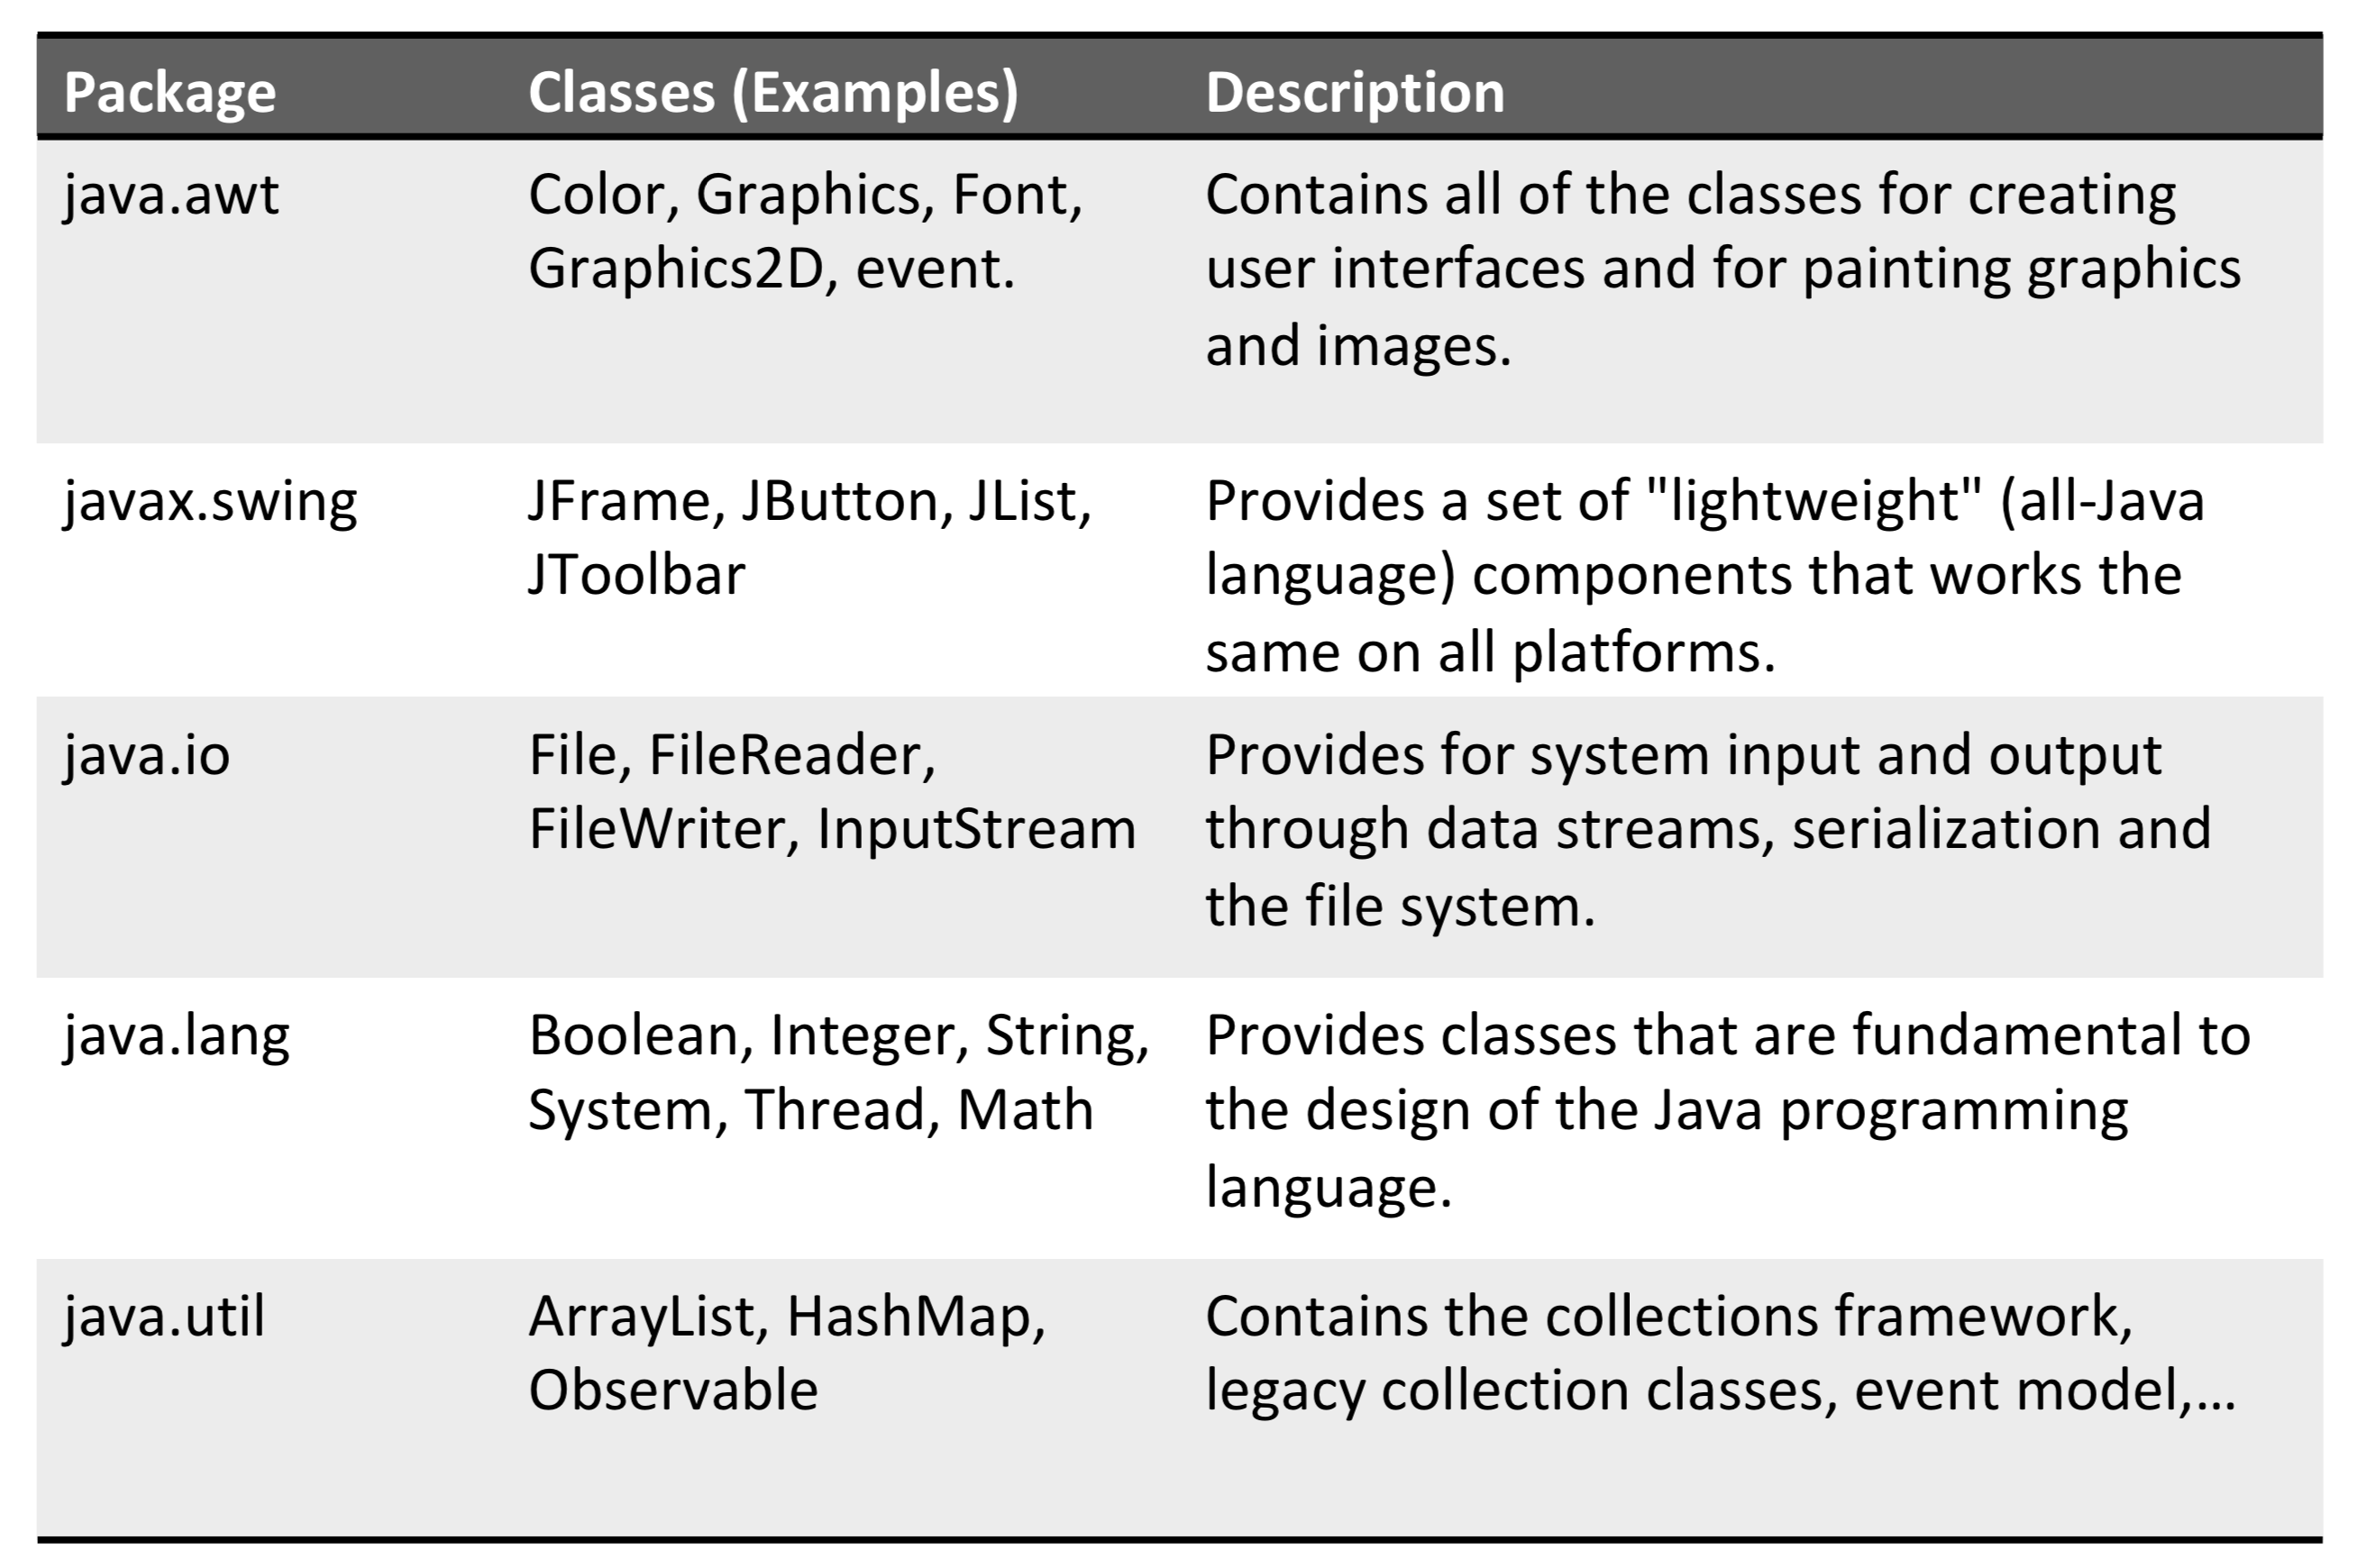
\includegraphics[scale=0.2]{11}\\
Taken from Lecture Notes
\end{center}

\subsection{Java Class Hierarchy}
\begin{itemize}
\item All classes (implicitly) derive from Object class (in java.lang) and has methods like clone(), toString(), finalize()
\item Classes you write inherit these basic behaviours
\end{itemize} 

\begin{center}
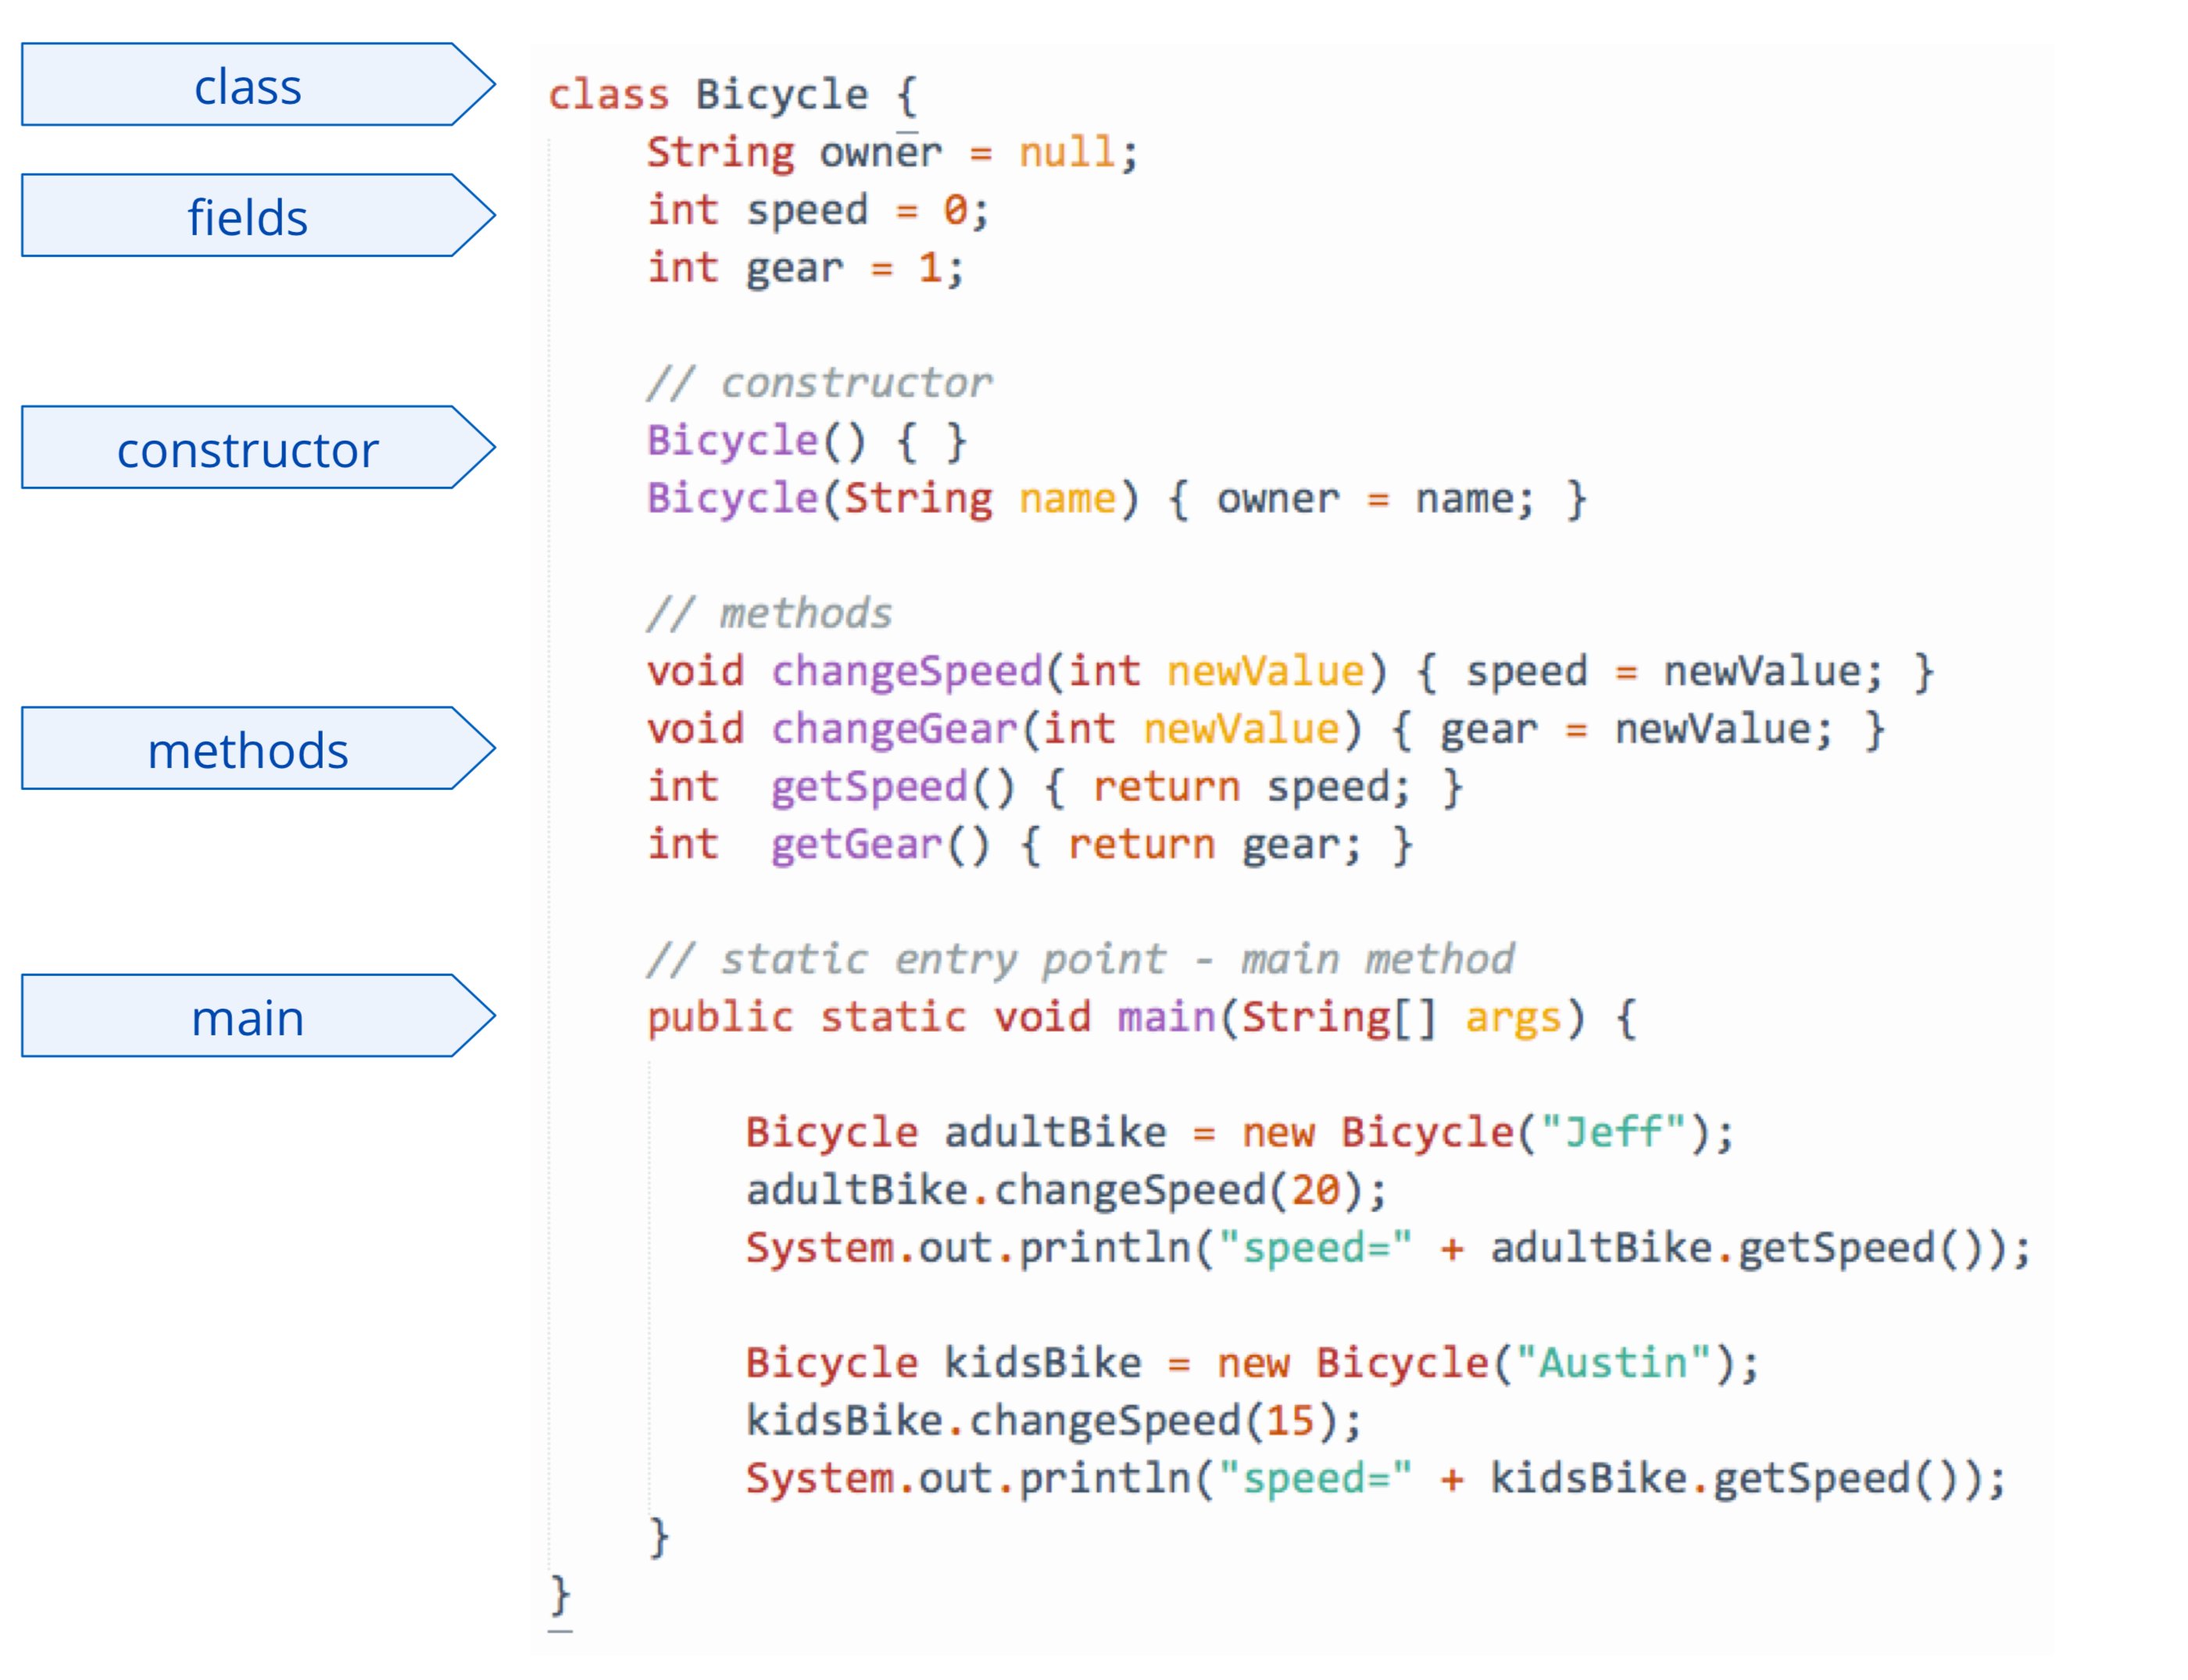
\includegraphics[scale=0.2]{12}\\
Taken from Lecture Notes
\end{center}

\subsection{Instantiating Objects}
\begin{itemize}
\item Primitive types (int, float, etc) are located on the stack and always passed by value
\item Objects are allocated on the heap and can be thought of as always passed by reference, but in truth object address is passed by value
\item There are no "pointer semantics" in Java
\end{itemize}

\subsection{Inheritance}
\begin{itemize}
\item Inherit some methods or fields from a base class ("is a") 
\item Its very common in Java to inherit and override other classes
\end{itemize}


\begin{center}
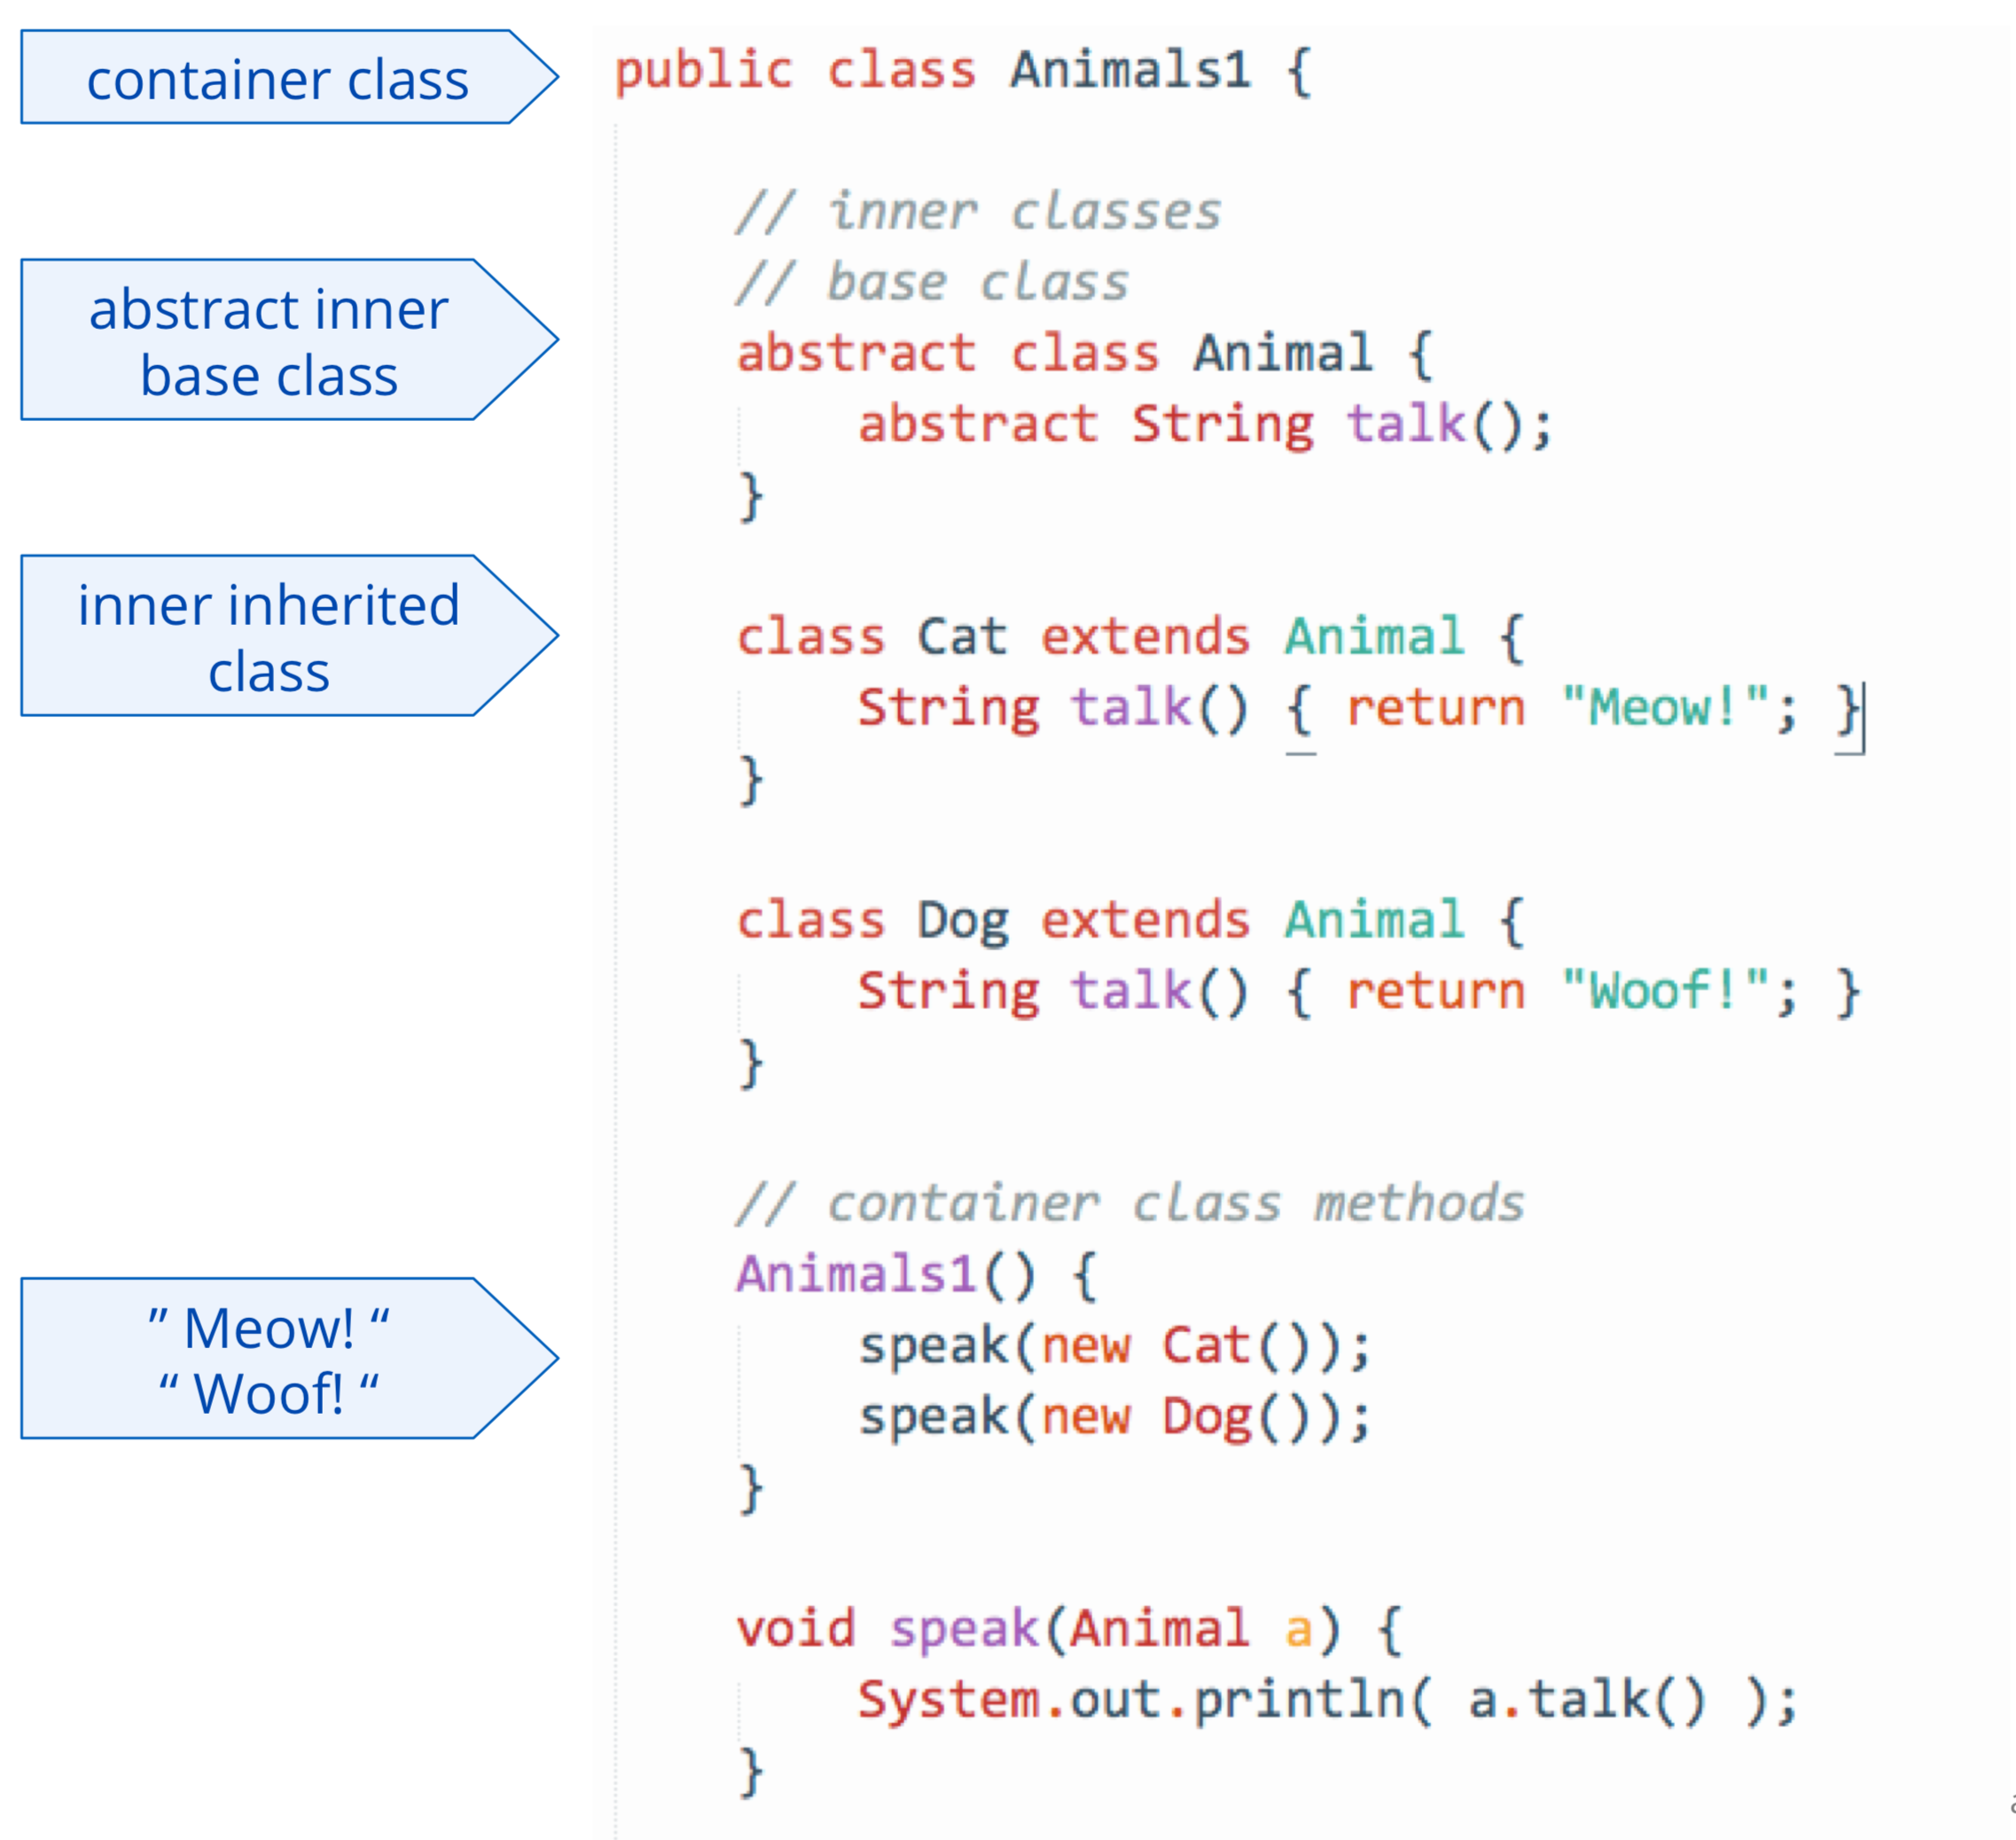
\includegraphics[scale=0.2]{13}\\
Taken from Lecture Notes
\end{center}

\subsection{Interfaces}
\begin{itemize}
\item An \verb|interface| represents a set of methods a class must have. Its basically a pure abstract class 
\item A class \verb|implements| "all" methods in the interface
\item A class can implement multiple interfaces
\item Interfaces are often used to enforce an API, not functionality 
\end{itemize}

\begin{center}
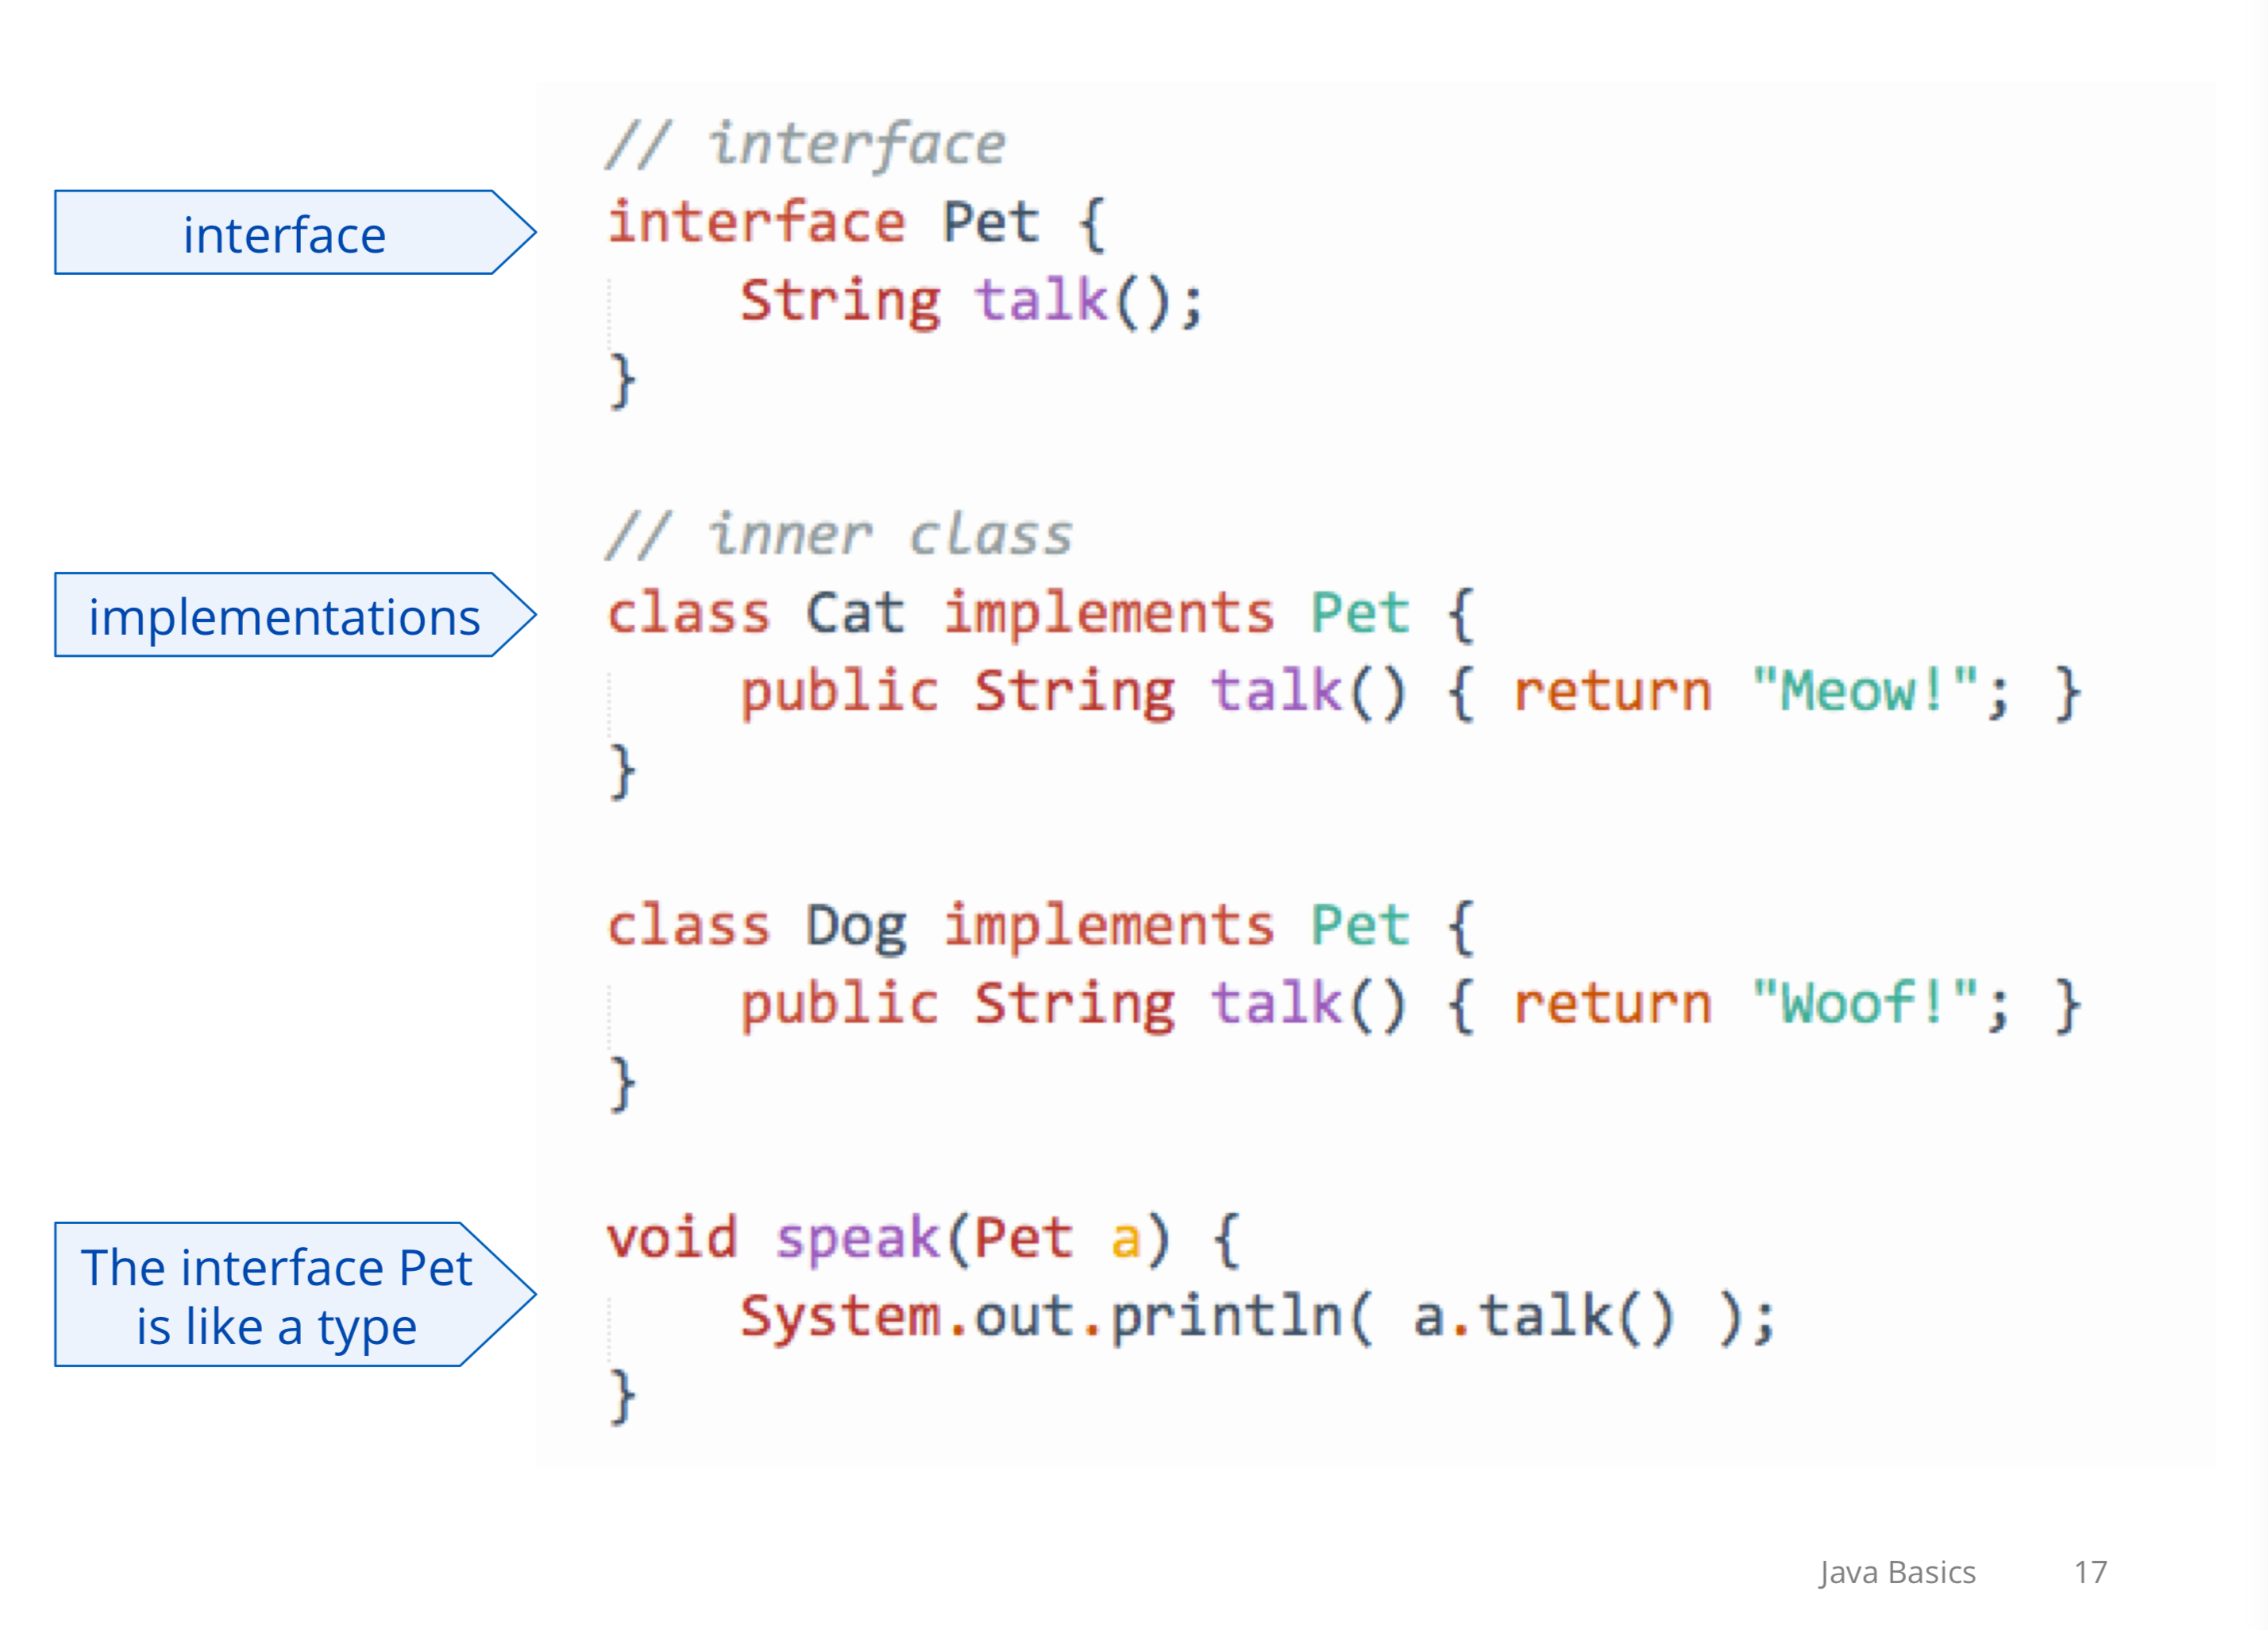
\includegraphics[scale=0.2]{14}\\
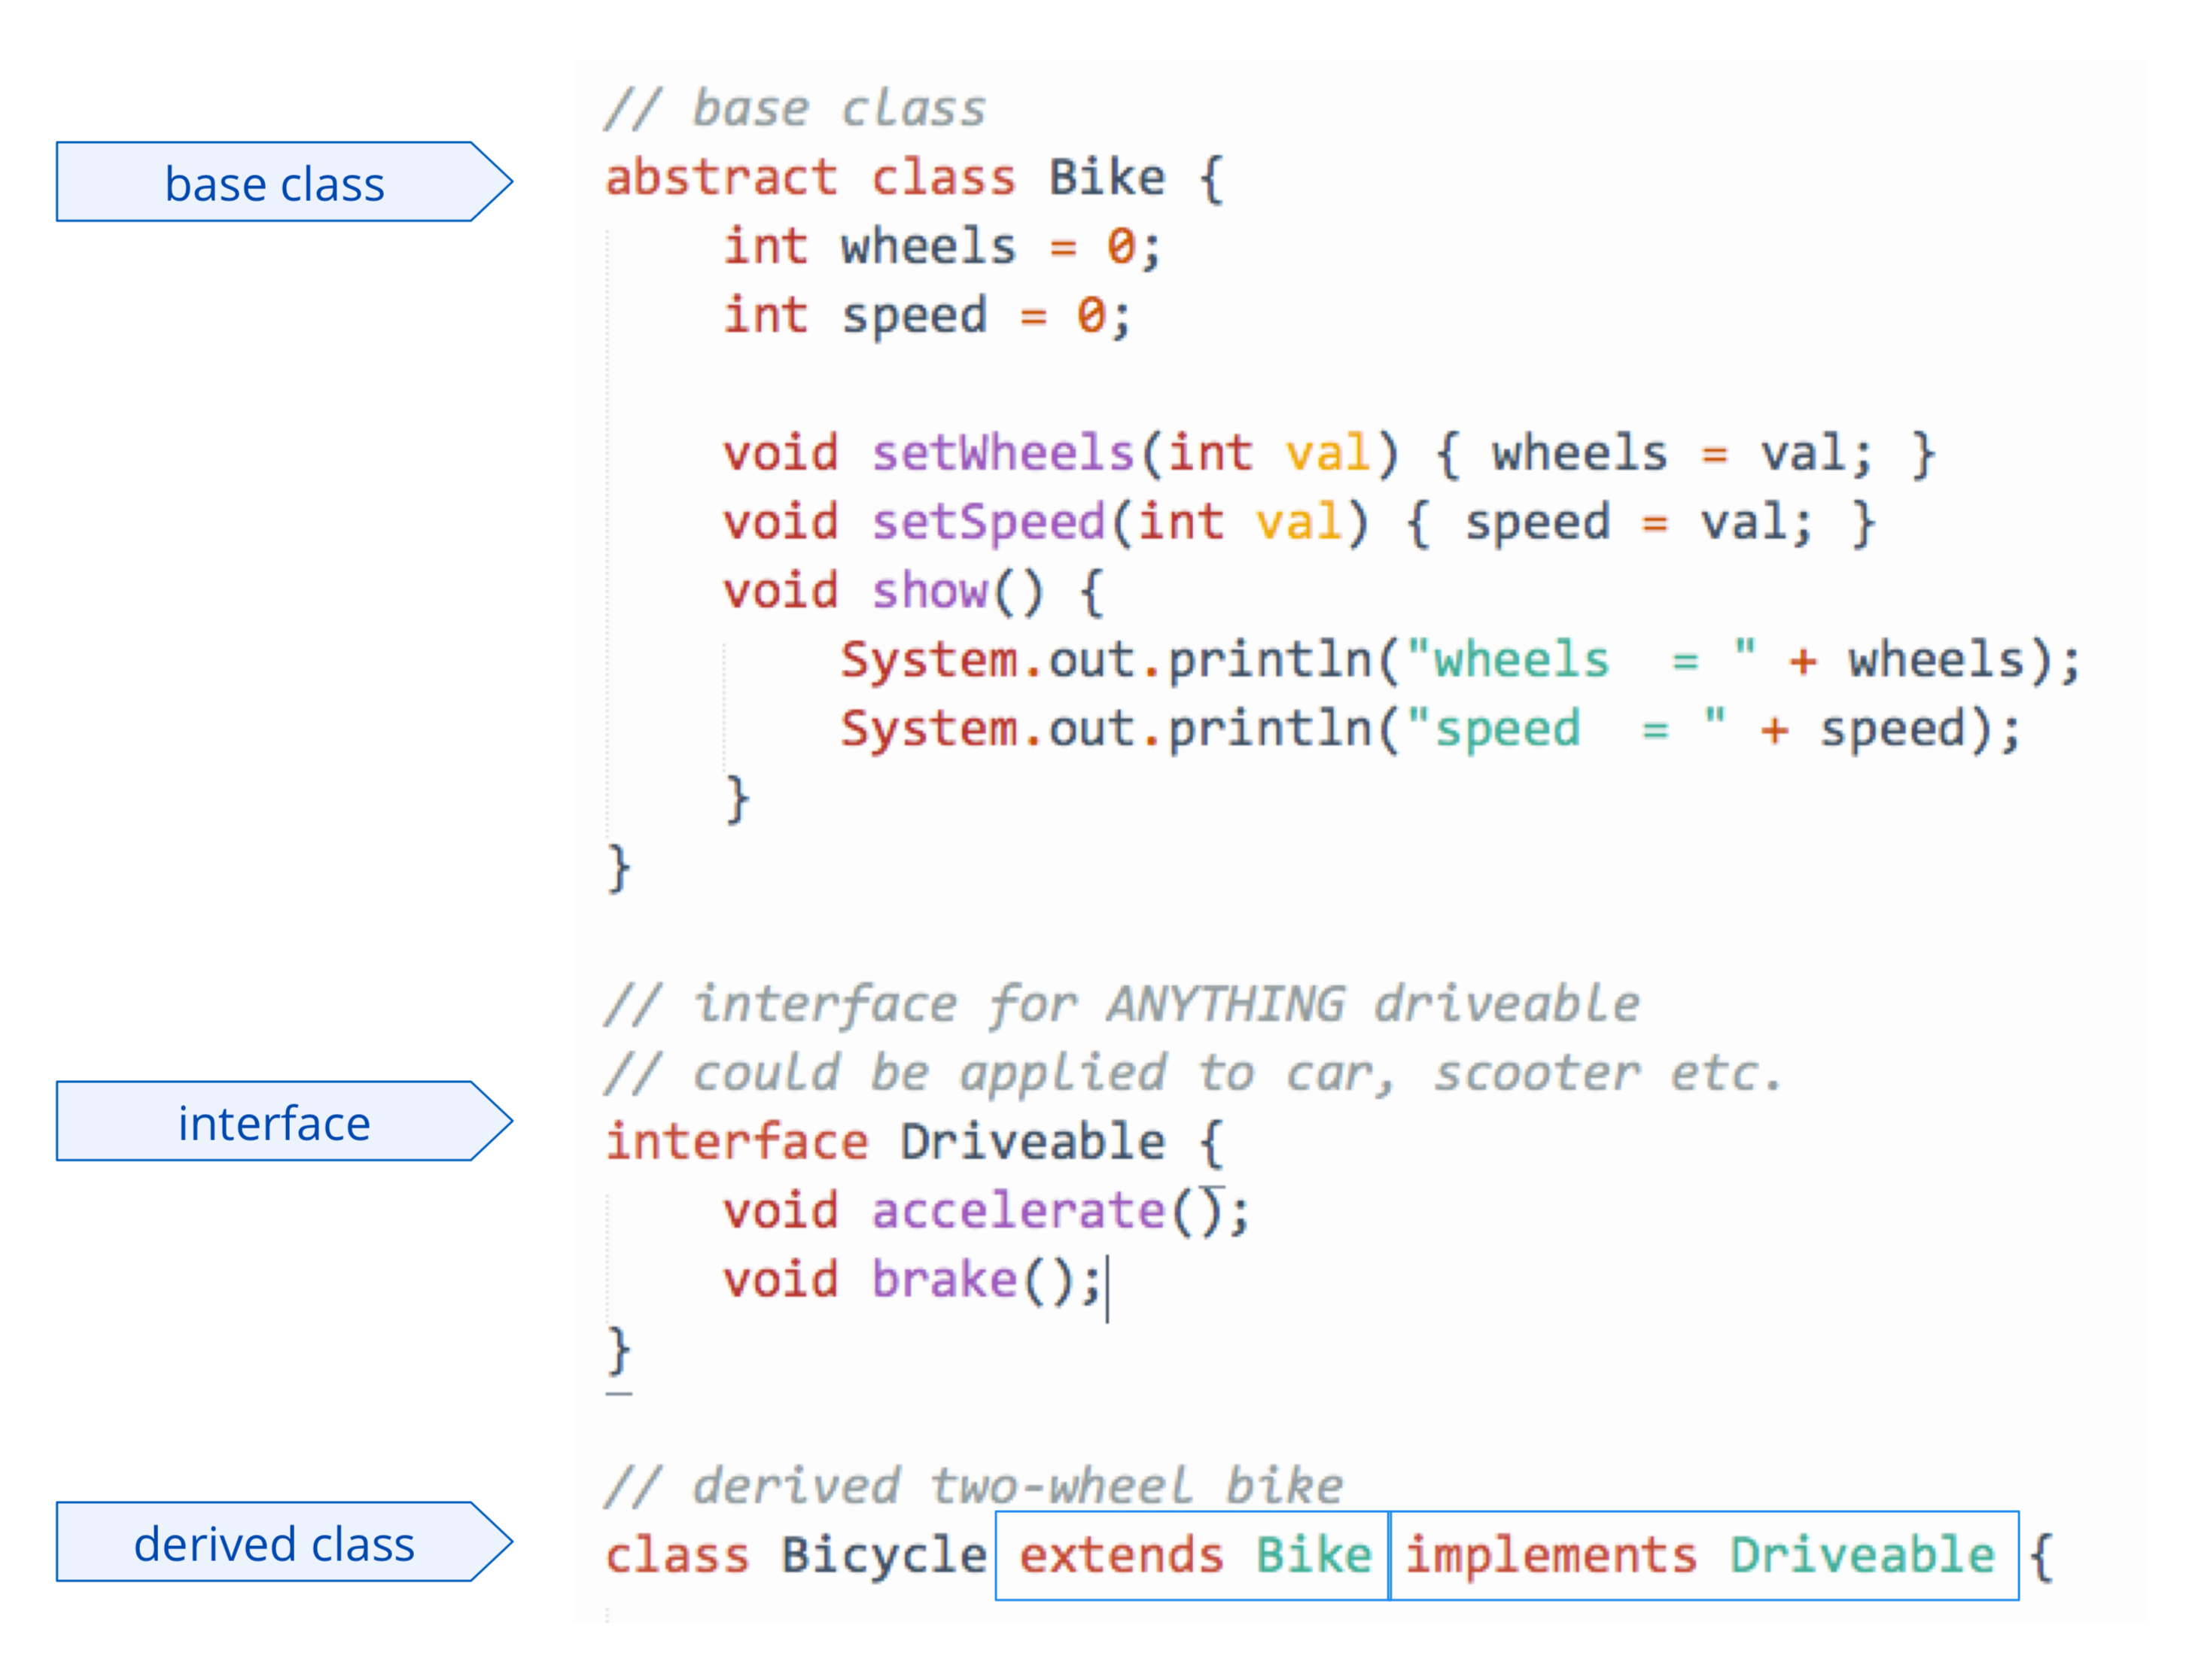
\includegraphics[scale=0.2]{15}\\
Taken from Lecture Notes
\end{center}


\end{document}





